\documentclass{beamer}
\usepackage[utf8]{inputenc}
\usepackage{graphics}
\usepackage{soul}
\mode<presentation> {
\usetheme{unc}}
\setbeamertemplate{navigation symbols}{} % To remove the navigation symbols from the bottom of all slides uncomment this line

\usepackage{graphicx} % Allows including images
\usepackage{booktabs} % Allows the use of \toprule, \midrule and \bottomrule in tables


\usepackage{hyperref}
\hypersetup{linkcolor=blue,colorlinks=true}


% Remove symbols
\beamertemplatenavigationsymbolsempty


%\usetheme{default}

\usefonttheme{serif}

%----------------------------------------------------------------------------------------
%	TITLE PAGE
%----------------------------------------------------------------------------------------


\title[Domestic Constraints and the Democratic Peace]{\LARGE{Domestic Constraints on War and the Democratic Peace}}
\author[POLI 150]{Steven Saroka}
\institute{POLI 150}
\date{6 February 2023}


\begin{document}

\begin{frame}
\titlepage % Print the title page as the first slide
\end{frame}

%----------------------------------------------------------------------------------------
%	PRESENTATION SLIDES
%----------------------------------------------------------------------------------------


%% Slide outline
\begin{frame} 
	\frametitle{\LARGE{Today's Class}}
	\begin{itemize}
		\Large{
			\item Putnam and Two-Level Games
			\\~\\ 
			\item Domestic Politics and War
			\\~\\ 
			\item Democratic Peace
		}
	\end{itemize}
\end{frame}

\begin{frame} 
	\frametitle{\LARGE{Reminders}}
	\begin{itemize}
		\Large{
			\item Prompt 4 due tonight; prompt 5 due Thursday.
		}
	\end{itemize}
\end{frame}

\begin{frame} 
	\frametitle{\LARGE{Central Question}}
	\centering
	\Large{How can domestic factors influence interstate war?}
\end{frame}

\begin{frame} 
	\frametitle{\LARGE{Key Terms}}
	\begin{itemize}
		\item Two-Level Game 
		\item Diversionary War
		\item Rally Effect
		\item Democratic Peace
	\end{itemize}
\end{frame}

%\begin{frame} 
%	\frametitle{\LARGE{Putnam Review}}
%	Group yourselves and answer the following:
%	\begin{itemize}
%		\item What was Putnam's main point?
%		\item What are the levels of the two-level game?
%		\item What is a win-set?
%		\item How does the two-level game impact international bargaining?
%	\end{itemize}
%\end{frame}

\begin{frame} 
\frametitle{\LARGE{Putnam and Two-Level Games}}
	\begin{itemize}
		\item Putnam claims that research focusing on just bargaining at the international level is incomplete. \pause
		\begin{itemize}
			\item The bargaining model of war implicitly focuses on the international level. \pause
		\end{itemize}
		\item Putnam's main insight is that \textbf{even when states are negotiating with each other, each side's diplomats must also remember domestic factors.} \pause
		\item Thus, he suggests that we should study \textbf{two-level games}: games where actors attempt to reach an agreement that is acceptable to an international bargaining partner \textbf{and} a domestic audience.
	\end{itemize}
\end{frame}

\begin{frame} 
	\frametitle{\LARGE{Putnam and Two-Level Games}}
	\begin{itemize}
		\item He uses game theory to model this as a \textbf{two-level game}: a model of international bargaining with domestic constraints. \pause
		\item This model has two levels:
		\begin{itemize}
			\item Level 1: International negotiations/bargaining. \pause
			\item Level 2: Domestic lobbying and constraints. \pause
		\end{itemize}
		\item We have been talking about Level 1 for the past few classes - the bargaining model of war is focused on this level. 
	\end{itemize}
\end{frame}

\begin{frame} 
	\frametitle{\LARGE{Putnam and Two-Level Games}}
	\begin{itemize}
		\item We have thus far assumed that states are \textbf{unitary actors}: actors with a single set of preferences.
		\item This model removes that assumption. \pause
		\item Actors now must find a negotiated settlement that is acceptable to \textbf{both}  the other state and their own domestic audience. \pause
		\item National leaders are negotiators with two other parties: their foreign counterpart and their own domestic constituents. 
	\end{itemize}
\end{frame}


\begin{frame} 
\frametitle{\LARGE{Two-Level Game Steps}}
	\begin{itemize}
		\item In this model, bargaining first takes place at the international level (Level 1) and then the domestic level (Level 2). \pause
		\item Negotiators/leaders can agree to a deal between their states at L1. \pause
		\item Each leader then takes that agreement to their domestic audiences to seek ratification. \pause
		\item Sometimes, this process is iterative, with leaders coming back to L1 for multiple revisions of the deal based on input from L2.
	\end{itemize}
\end{frame}

\begin{frame} 
\frametitle{\LARGE{Win-Sets}}
	\begin{itemize}
		\item Each leader will only accept a deal within their \textbf{win-set}. \pause
		\item \textbf{Win-set}: the range of international agreements that will be accepted at the domestic level. \pause
		\item Larger win-sets thus make agreements more likely. \pause
		\item The size of domestic win-sets affects the distribution of outcomes possible in international bargaining.
	\end{itemize}
\end{frame}

\begin{frame} 
\frametitle{\LARGE{Changing Win-Sets}}
\begin{figure}[ht!]
	\centering
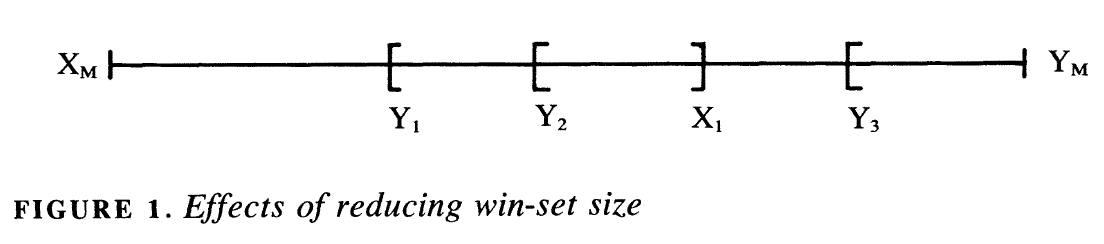
\includegraphics[width=\textwidth,height=0.8\textheight,keepaspectratio]{./winset.png}
\end{figure}
\end{frame}

\begin{frame} 
\frametitle{\LARGE{Determinants of Win-Set Size}}
 What determines how large or small a win-set is? \pause
	\begin{enumerate}
		\item Status-quo or reversion point: what do leaders stand to gain? What happens if they fail to reach any deal? \pause
		\item The distribution of domestic actors: are they homogeneous or heterogeneous?    \pause 
		\item Issue linkage: what are the dimensions of bargaining? \pause 
		\item Institutions: how are agreements ratified by the domestic audience?
	\end{enumerate}
\end{frame}

\begin{frame} 
	\frametitle{\LARGE{Two-Level Games}}
		\begin{itemize}
			\item The introduction of a second level means that `wrong' decisions become doubly likely. \pause
			\item The other state's leader can inflict costs on the opposing state. \pause
			\item Domestic actors unhappy with a deal can remove the national leader from power. \pause
			\item \textbf{When acting internationally, outcomes must please both international and domestic actors.}
		\end{itemize}
\end{frame}

\begin{frame} 
	\frametitle{\LARGE{Strategic Interaction in Two-Level Games}}
	\begin{itemize}
		\item L1 actors are especially uncertain about the L2 domestic considerations of their counterparts. \pause
		\item This uncertainty is both a bargaining tool and a constraint. \pause
		\item Each L1 has an incentive to understate the domestic side of their win-set, but also knows this about the other side. \pause
		\item This uncertainty increases risk of involuntary defection by the other side if their L2 supporters won't ratify a deal, so L1 negotiators want to be certain any deal is within the other side's L2 win-set. \pause
		\item This means they may not press for especially harsh bargains that the other side's L2 won't accept.
	\end{itemize}
\end{frame}

\begin{frame} 
	\frametitle{\LARGE{Two-Level Games Wrap-Up}}
	\begin{itemize}
		\item This model illustrates that no state or leader is independent from its domestic politics.
		\item The internal domestic institutions thus influence how international bargaining and cooperation plays out by impacting the bargaining range. \pause
		\item Opaque domestic institutions make it harder for other states to determine resolve.  \pause 
		\item The need to obey domestic coalitions may make it harder for states to commit to agreements.
	\end{itemize}
\end{frame}

\begin{frame} 
	\frametitle{\LARGE{Two-Level Games Wrap-Up}}
	\begin{itemize}
		\item While we often consider states to be \textbf{unitary actors}, that is an assumption that can sometimes obscure important details. \pause
		\item We must consider both the international and domestic incentives that actors face to study their decision-making. \pause
		\item\textbf{We have already discussed international incentives with the bargaining model of war, so what do these L2 domestic incentives look like?}
	\end{itemize}
\end{frame}


\begin{frame} 
	\frametitle{\LARGE{Domestic Politics and War: Gas}}
	\begin{figure}[ht!]
		\centering
		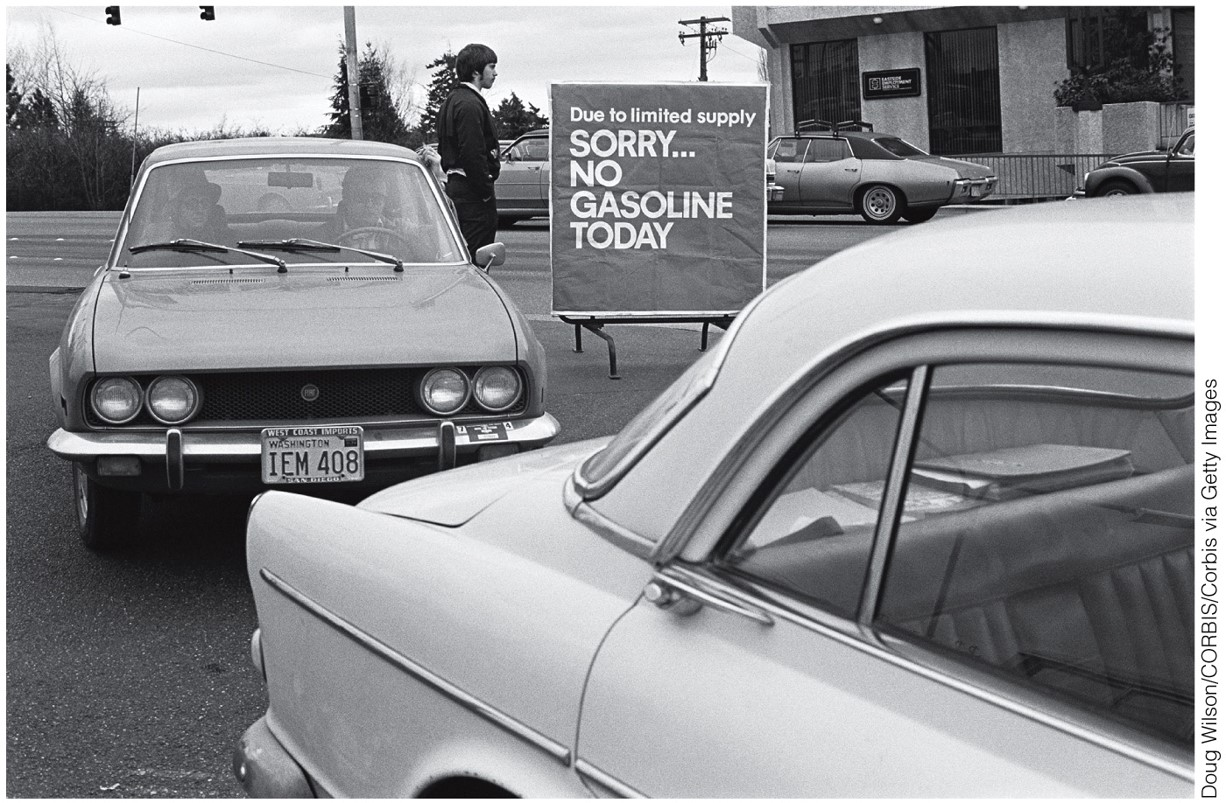
\includegraphics[width=\textwidth,height=0.9\textheight,keepaspectratio]{Gasshort.jpg}
	\end{figure}
\end{frame}

\begin{frame} 
	\frametitle{\LARGE{Domestic Politics and War: Oil Price}}
	\begin{figure}[ht!]
		\centering
		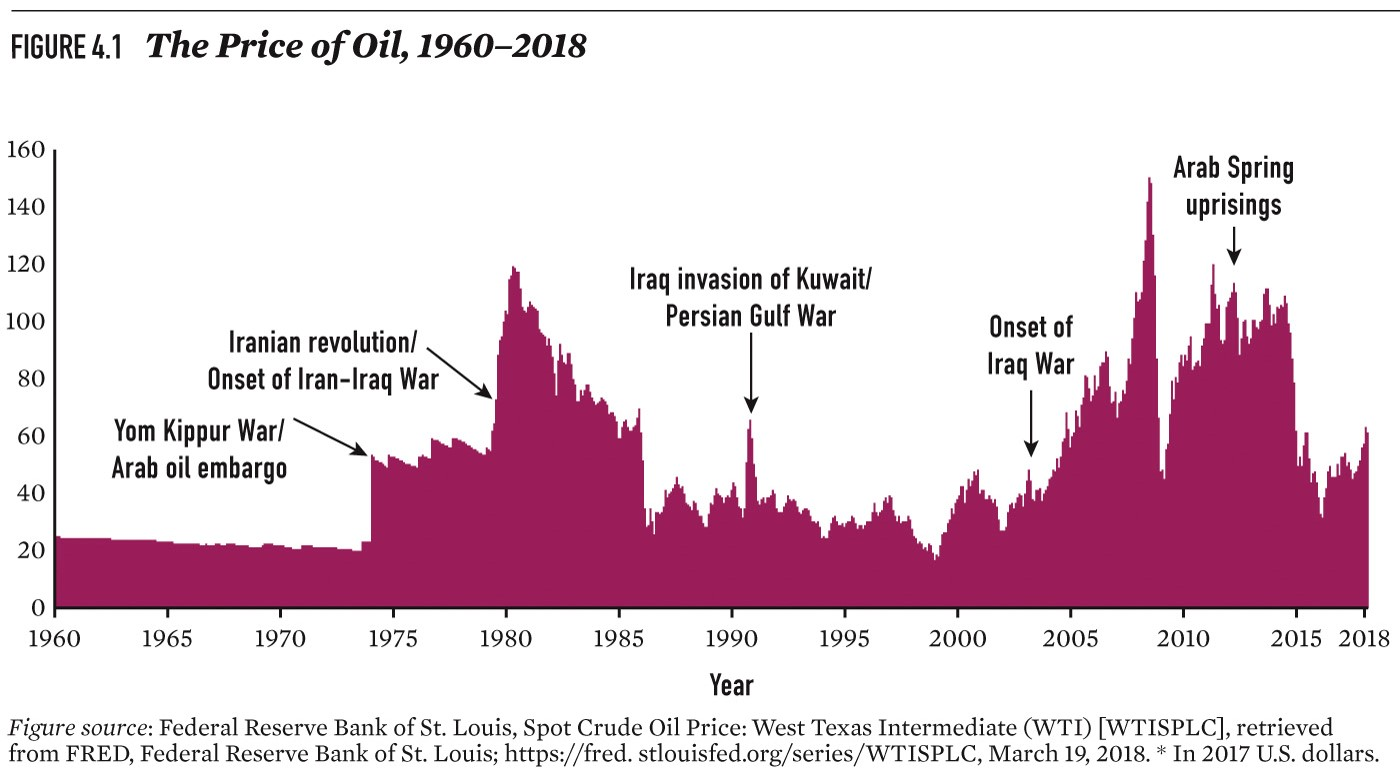
\includegraphics[width=\textwidth,height=0.9\textheight,keepaspectratio]{Oilpricewar.jpg}
	\end{figure}
\end{frame}

\begin{frame} 
	\frametitle{\LARGE{Domestic Politics and War: Oil Price}}
	\begin{itemize}
		\item US consumer dependence on gasoline means that US consumers have an interest in stability in the Middle East. \pause
		\item Some have argued that, due to this dependence of both the military and civilian economy, US interventions in the ME are in the national interest. \pause
		\item This is a specific example of how internal (L2) domestic characteristics can influence military commitments (such as placement of US military bases in the ME) or political commitments (such as US-Saudi Arabia alliance).
	\end{itemize}
\end{frame}

\begin{frame} 
	\frametitle{\LARGE{Domestic Politics and War: Interests}}
	\begin{itemize}
		\item More generally, this shift to considering L2 means that we are shifting away from national interests in war towards considering particularistic interests in war. \pause
		\item \textbf{National interests}: the motivations of states so far (power, security, wealth). \pause
		\item \textbf{Particularistic interests}: the motivations of specific groups within states. \pause
		\item Who are these groups?
	\end{itemize}
\end{frame}

\begin{frame} 
	\frametitle{\LARGE{Domestic Actors}}
	\begin{figure}[ht!]
		\centering
		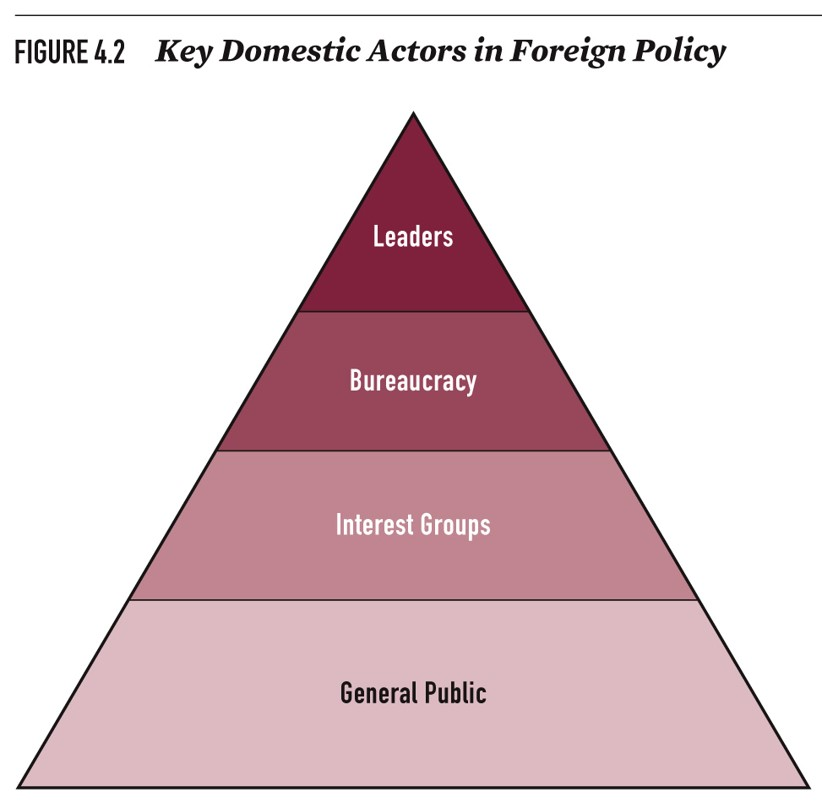
\includegraphics[width=\textwidth,height=0.9\textheight,keepaspectratio]{Domesticactors.jpg}
	\end{figure}
\end{frame}

\begin{frame} 
	\frametitle{\LARGE{Domestic Actors: Leaders}}
 Do leaders ever spark war to generate domestic benefits?
	\begin{figure}[ht!]
	\centering
	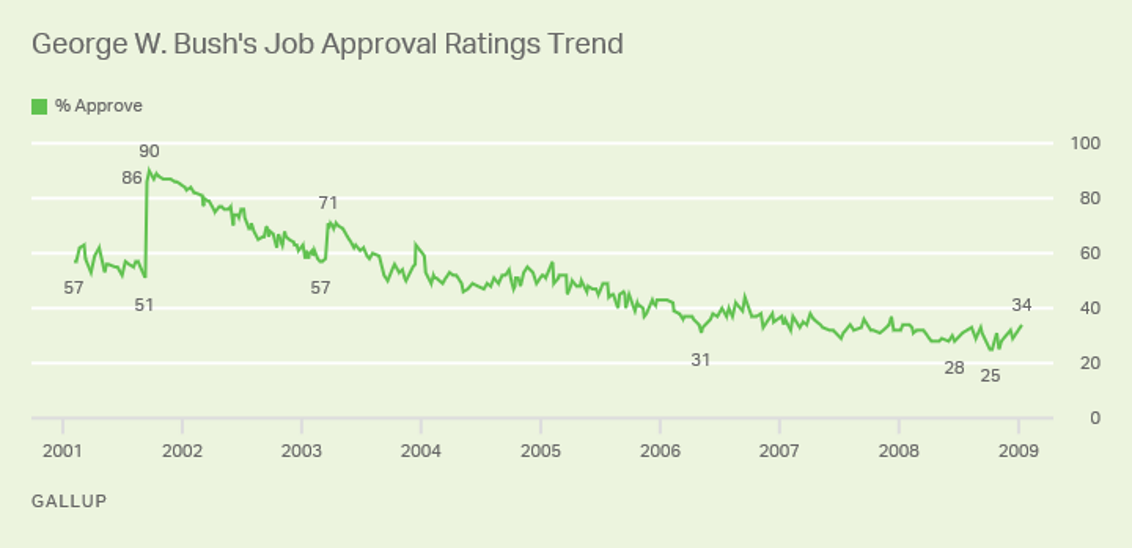
\includegraphics[width=\textwidth,height=0.9\textheight,keepaspectratio]{Bushapproval.png}
	\end{figure}
\end{frame}

\begin{frame} 
	\frametitle{\LARGE{Domestic Actors: Leaders}}
	\begin{itemize}
		\item One common explanation for war: leaders will start a war to generate a “rally around the flag.” \pause
		\item \textbf{Rally effect}: temporary increase in citizen support for their state's government in response to international crises or wars. \pause
		\item This can yield particularistic benefits to the leader, such as boosting support. \pause
		\begin{itemize}
			\item Benefits for both democratic and autocratic leaders: reelection or increased legitimacy.
		\end{itemize}
		\item Existence of rally effects creates a \textbf{diversionary incentive} for leaders. 
		\item How does this impact the bargaining range?
	\end{itemize}
\end{frame}

\begin{frame} 
	\frametitle{\LARGE{Rally Effects and Bargaining Range}}
	\begin{figure}[ht!]
		\centering
		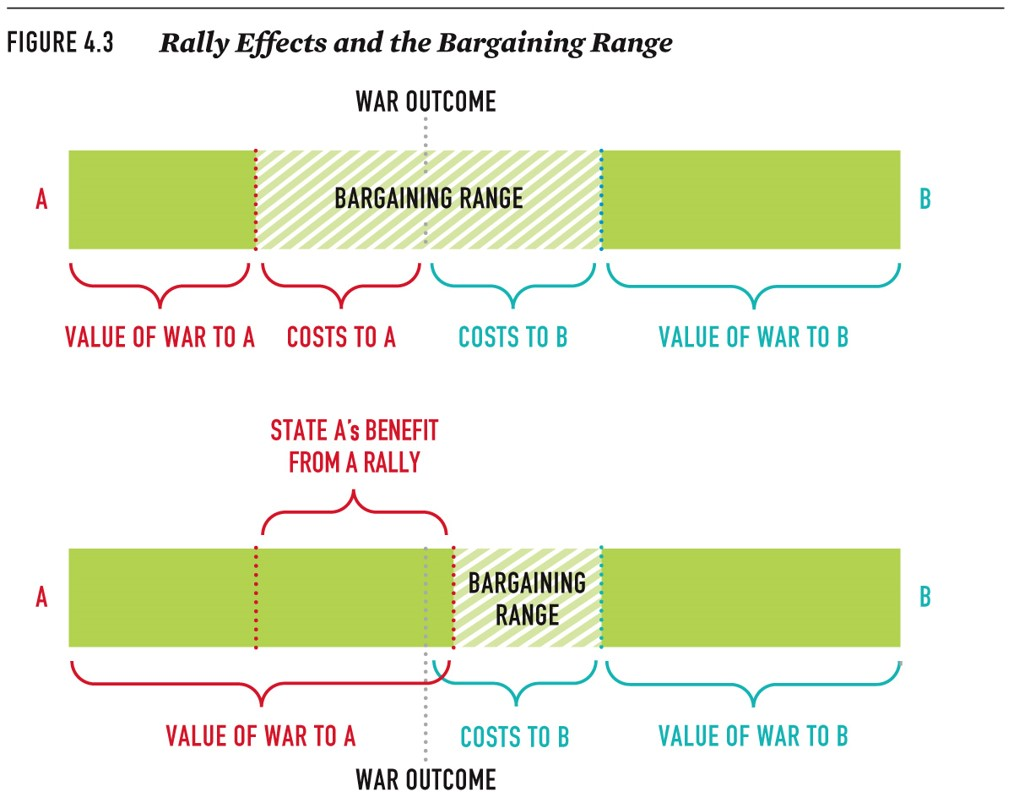
\includegraphics[width=\textwidth,height=0.9\textheight,keepaspectratio]{Rallyeffectsbarg.jpg}
	\end{figure}
\end{frame}

%https://www.ft.com/content/fccc5384-4dc8-11e2-a0fc-00144feab49a
\begin{frame} 
	\frametitle{\LARGE{Rally Effects: Falkland Islands War}}
	\begin{figure}[ht!]
		\centering
		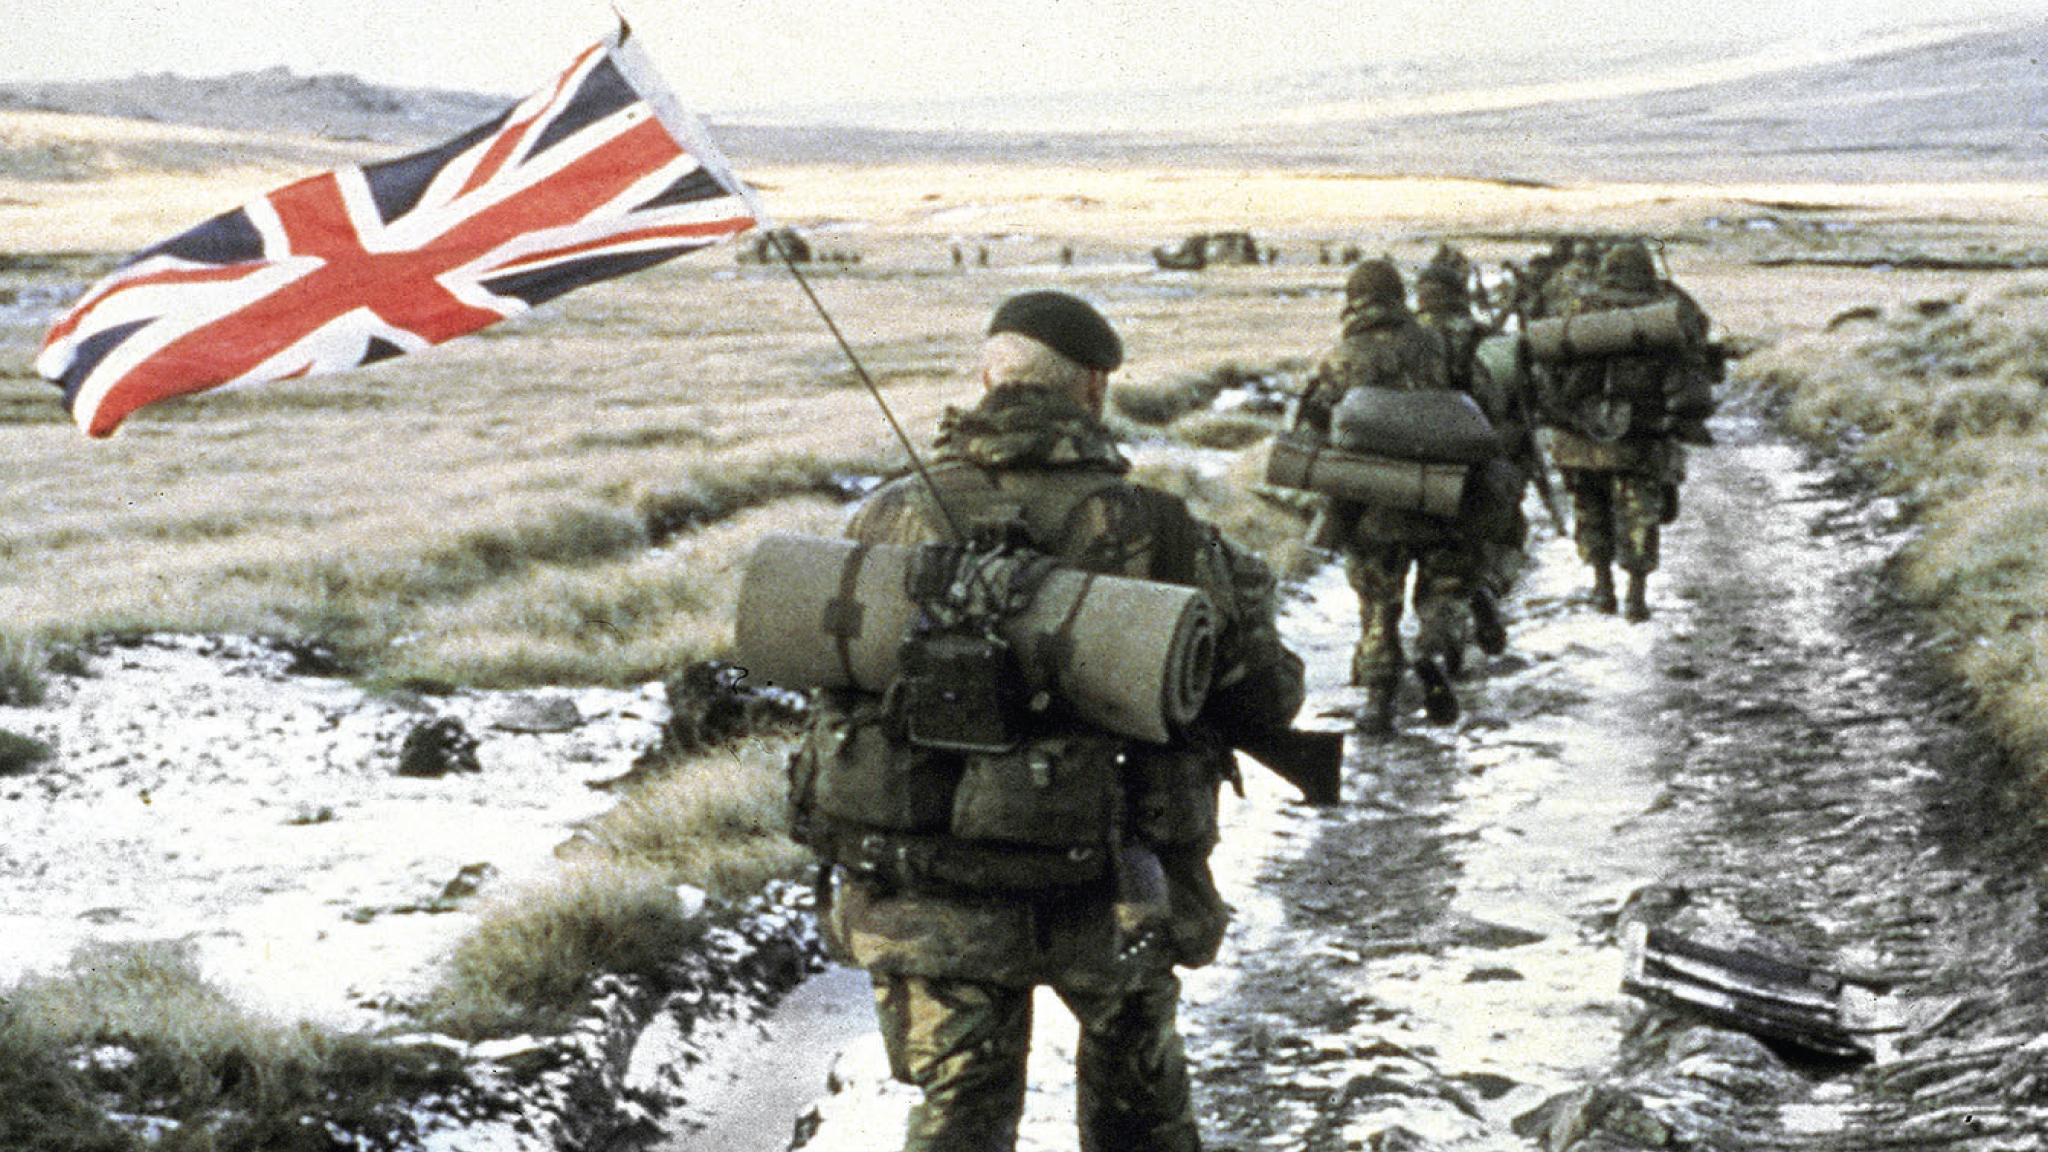
\includegraphics[width=\textwidth,height=0.9\textheight,keepaspectratio]{Britishtroops.jpg}
	\end{figure}
\end{frame}

\begin{frame} 
	\frametitle{\LARGE{Rally Effects: Falkland Islands War}}
	\begin{itemize}
		\item Argentine ruling junta facing domestic riots and demands for its overthrow. \pause
		\item Seizing the Falkland Islands, a British possession, shifted the Argentine public's attention away from that domestic discontent (temporarily). \pause
		\item Britain experiencing economic recession, and PM Thatcher facing very low approval ratings. \pause
		\item Thatcher received a substantial boost in her approval ratings following the start of the war, which lasted Apr. 2 - Jun. 14, 1982 and ended in British victory.
	\end{itemize}
\end{frame}

\begin{frame} 
	\frametitle{\LARGE{Rally Effects Wrap-Up}}
	\begin{itemize}
		\item Like the brinksmanship strategy, rally effects tend to lack systematic evidence for their use outside of a few high-profile examples. \pause
		\item Benefits of war must certainly outweigh benefits of peace for a rational leader to launch a war in hopes of rally effect, which is rare. \pause
		\item Rally effects are also temporary, as support decreases as casualties rise.
	\end{itemize}
\end{frame}

\begin{frame} 
	\frametitle{\LARGE{Rally Effects Wrap-Up}}
	\begin{figure}[ht!]
		\centering
		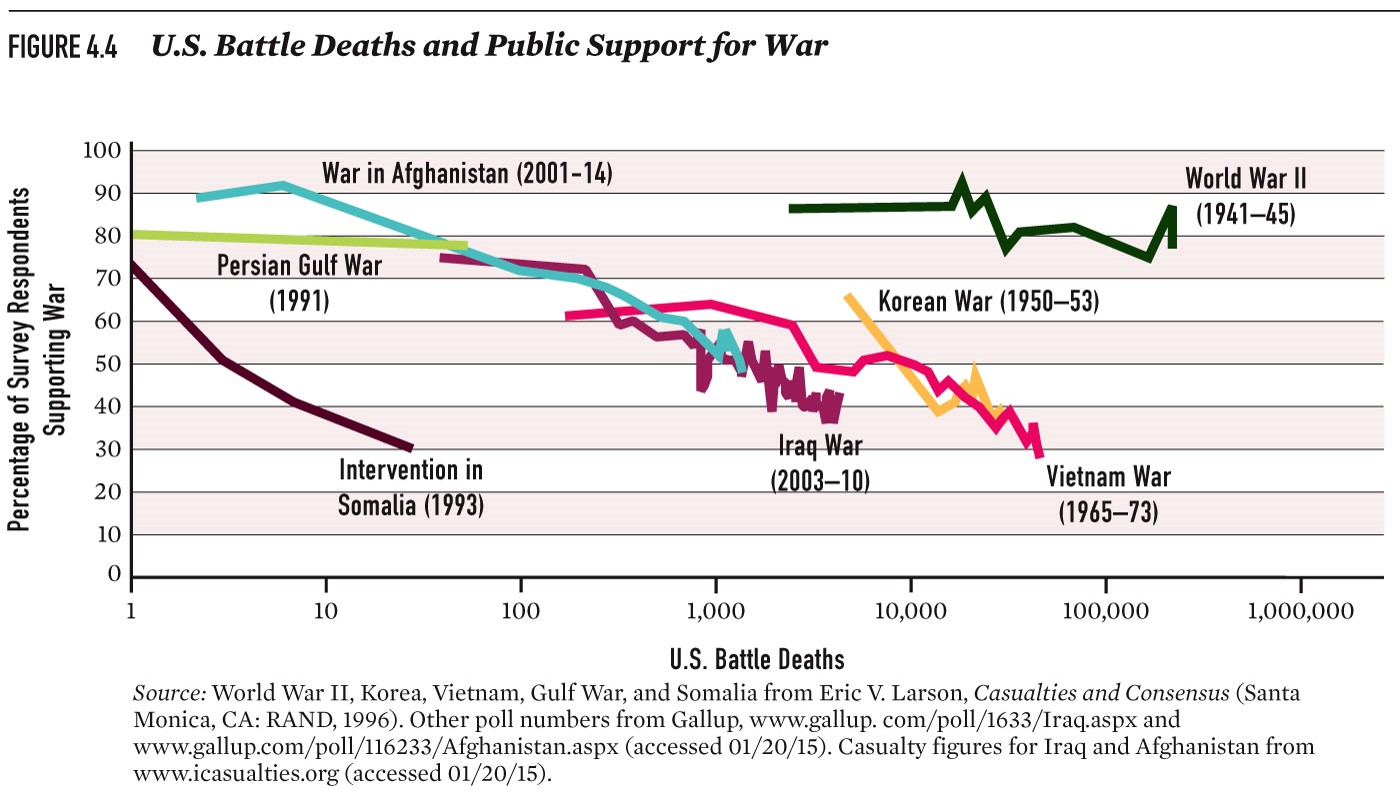
\includegraphics[width=\textwidth,height=0.9\textheight,keepaspectratio]{USappbd.jpg}
	\end{figure}
\end{frame}

\begin{frame} 
	\frametitle{\LARGE{Other Domestic Actors}}
	\begin{itemize}
		\item Other domestic actors, like the state's \textbf{bureaucracy} (including its military) and \textbf{interest groups}, may have particularistic interests in interstate war. \pause
		\begin{itemize}
			\item Military officers may view war as a chance for promotion and larger budget. \pause
			\item Military-industrial complex may view war as a chance for lucrative contracts. \pause
		\end{itemize}
	\item However, by definition, many of these groups will be much smaller than the general population who pay the costs of war (higher taxes and deaths). Why does their influence matter? 
	\end{itemize}
\end{frame}

\begin{frame} 
	\frametitle{\LARGE{Collective Action Problems Reprise}}
	\begin{itemize}
		\item This is a case of the bureaucracy and interest groups overcoming a collective action problem, while the general population cannot. \pause
		\item Recall the elements of successful collective action: smaller group size enables easier coordination and monitoring to prevent free-riding to obtain a public good. \pause
		\item In this case, the bureaucracy and special interest groups are sufficiently small that they can coordinate to effectively lobby government policy, gaining those benefits of war (``public goods" if we define ``public" as these groups).
		\item By contrast, the general population will struggle to mobilize for similar collective action reasons.
	\end{itemize}
\end{frame}

\begin{frame} 
	\frametitle{\LARGE{Collective Action Problems Reprise}}
	\begin{itemize}
		\item The costs of war fall on the general public, while the benefits accrue to the bureaucracy and special interest groups. \pause
		\item Note that this does not always mean the military is automatically warmongering: it can have a more realistic understanding of its costs and abilities than civilians. \pause
		\item More generally, this points to the idea that different groups with different preferences over war influence the bargaining range between two states, even if none of those groups are directly negotiating with the opposing side.
	\end{itemize}
\end{frame}

%\begin{frame} 
%	\frametitle{\LARGE{Domestic Actors and War}}
%	\begin{itemize}
%		\item Imagine there are two (generic) types of domestic actors in a state: \pause
%	\begin{itemize}
%		\item Hawks favor war.
%		\item Doves oppose war.
%	\end{itemize}
%		\item Say that only one type is in power at any given time. \pause
%		\item Which should expect higher costs from war?		
%	\end{itemize}
%\end{frame}

%\begin{frame} 
%	\frametitle{\LARGE{Hawks and Doves}}
%	\begin{figure}[ht!]
%		\centering
%		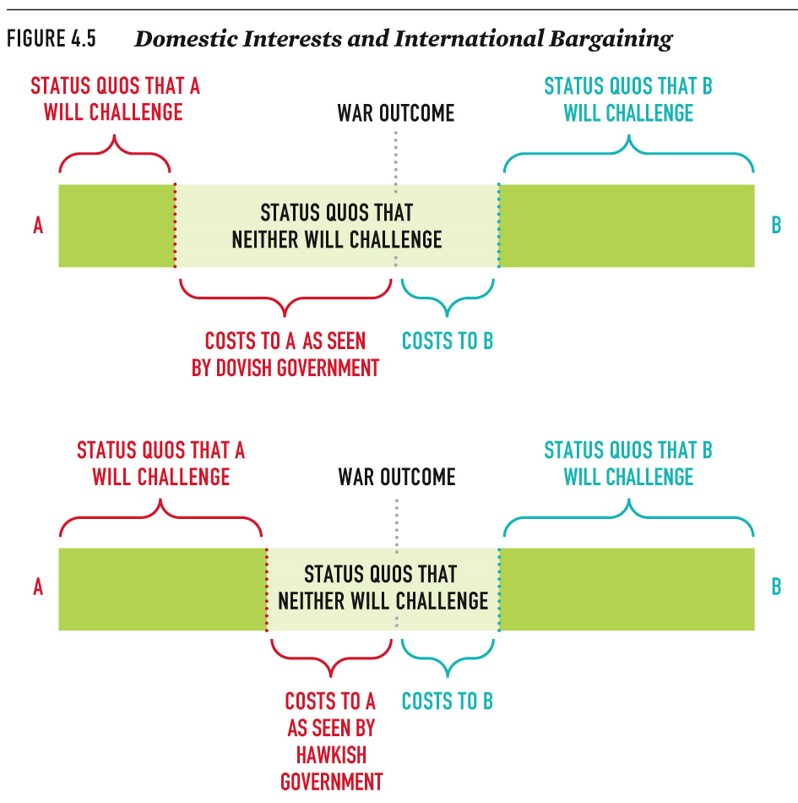
\includegraphics[width=\textwidth,height=0.9\textheight,keepaspectratio]{hawkdove.jpg}
%	\end{figure}
%\end{frame}

\begin{frame} 
\frametitle{\LARGE{Democratic Peace}}
\centering 
\Large{
	How does regime type (democracy or autocracy) influence war? 
}
\end{frame}

\begin{frame} 
\frametitle{\LARGE{The Decline in Conflict}}
\begin{figure}[ht!]
	\centering
	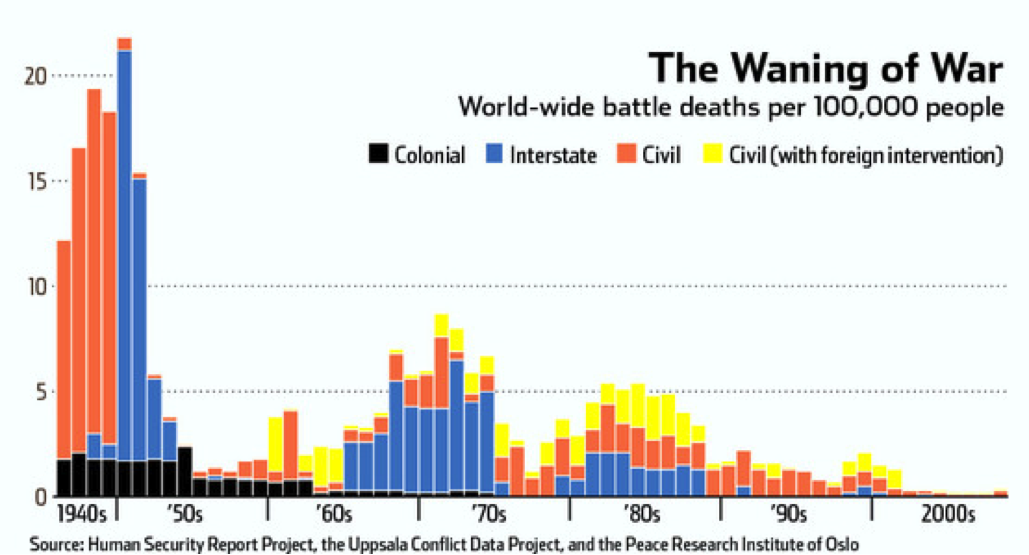
\includegraphics[width=\textwidth,height=0.8\textheight,keepaspectratio]{./waning_war.png}
\end{figure}
\end{frame}

\begin{frame} 
\frametitle{\LARGE{The Long Peace}}
\begin{itemize}
		\item Zero: the number of times nuclear weapons have been used since 1945 \pause

		\item Zero: Number of US-USSR wars \pause

		\item \st{Zero: Number of interstate wars in Europe since 1945}

		\item \st{Zero: Number of interstate wars in global north since 1945}
\pause

		\item Zero: Number of colonial conquests since 1945
\pause

		\item Zero: Number of states that disappeared due to conquest since 1945
\end{itemize}
\end{frame}

\begin{frame} 
\frametitle{\LARGE{Why the Long Peace?}}
\begin{itemize}
	\large{
		\item Given how bloody the first half of the 20th century was, why are we experiencing a long stretch of relative peace now? \pause 
		\item This observation sparked a substantial debate. \pause 
        \item The dominant answer is the \textbf{democratic peace}: the observation that democracies do not fight one another. \pause 
	    \item The democratic peace is held up as the closest thing in IR to a scientific law.
	}
\end{itemize}
\end{frame}

\begin{frame} 
	\frametitle{\LARGE{Spread of Democracy}}
	\begin{figure}[ht!]
		\centering
		\includegraphics[width=\textwidth,height=0.8\textheight,keepaspectratio]{Demspread.jpg}
	\end{figure}
\end{frame}

\begin{frame} 
\frametitle{\LARGE{The Democratic Peace}}
\begin{itemize}
		\item Modern democracies almost never fight wars with one another. \pause 
		\item However, democracies are \emph{not} less belligerent overall. \pause 
		\item Modern democracies are not less likely to go to war with non-democracies. \pause
		\item Policymakers clearly think it's important (e.g. Bush \& Obama statements)
\end{itemize}
\end{frame}

\begin{frame} 
\frametitle{\LARGE{What is a Democracy?}}
\begin{itemize}
	\large{
		\item Regime type refers to the type of government within each state. \pause 
		\item Generally divided into democracies and autocracies (non-democracies). \pause 
		\item \textbf{Democracy}: a political system in which candidates compete in frequent free and fair elections in which many can vote. \pause 
		\item \textbf{Autocracy}: a system in which power is concentrated in an individual or small group of people with no competition and few constraints on power. \pause 
		\item These are not perfectly measured concepts!
	}
\end{itemize}
\end{frame}

\begin{frame} 
\frametitle{\LARGE{Regime Type Around the World}}
\begin{figure}[ht!]
	\centering
	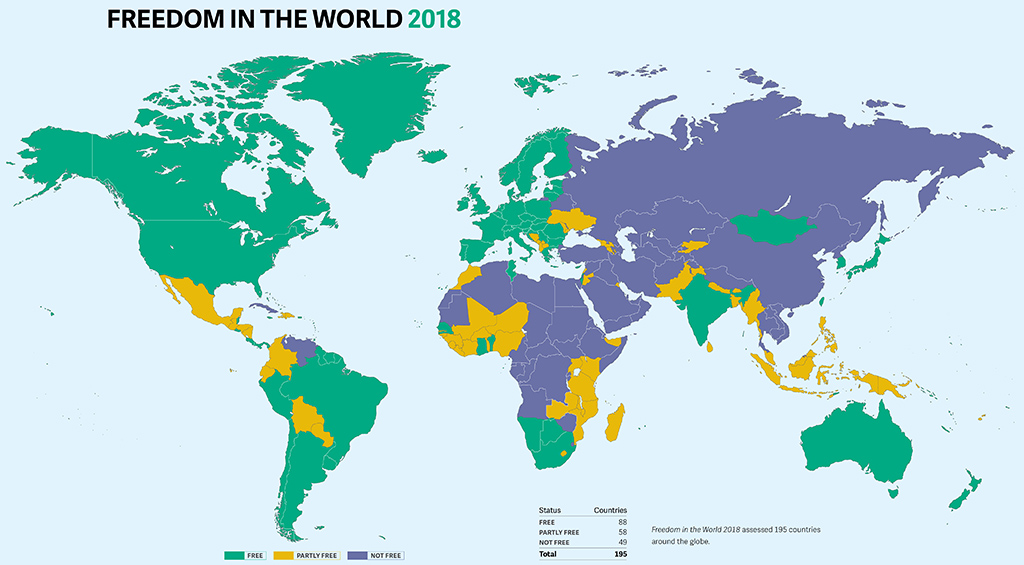
\includegraphics[width=\textwidth,height=0.8\textheight,keepaspectratio]{./democ.jpg}
\end{figure}
\end{frame}

\begin{frame} 
\frametitle{\LARGE{Why the Democratic Peace?}}
What are the proposed explanations for the democratic peace? \pause
\begin{enumerate}
		\item Norms of mutual respect and nonviolence. \pause 
		\item Democratic institutional impacts on the bargaining process. \pause
		\item The relationship is spurious (something else explains it).
\end{enumerate}
\end{frame}

\begin{frame} 
	\frametitle{\LARGE{Explanation 1: Norms}}
	\begin{itemize}
		\item One proposed explanation for the democratic peace is the norms of mutual respect and nonviolence. \pause 
		\item The idea here is that democracies are, by their nature, just less aggressive and prone to resorting to violence. \pause
		\item This explanation is not convincing, as data shows democracies are not less likely to go to war with non-democracies.
	\end{itemize}
\end{frame}

\begin{frame} 
\frametitle{\LARGE{Explanation 2: Institutions}}
\begin{itemize}
		\item In democracies, leaders are accountable to the public. \pause
		\item In autocracies, leaders are accountable to small groups of elites that keep them in power. \pause
		\item The degree to which the ``selectorate'' (the group keeping them in power) holds leaders accountable constrains their decisions. \pause
		\item \textbf{Accountability}: the ability to punish or reward leaders for their decisions.

\end{itemize}
\end{frame}


\begin{frame} 
\frametitle{\LARGE{Explanation 2: Institutions}}
\begin{itemize}
		\item Because of accountability, democratic leaders have systematically higher costs for war. \pause 
		\item War is thus less attractive, meaning that they will challenge fewer status quo situations. \pause
		\item Democratic leaders should only start wars that they are very likely to win. \pause 
		\item These things make war between democracies especially unlikely. \pause 
		\item Does not affect autocracies challenging democracies (e.g. Persian Gulf War and Pearl Harbor)
\end{itemize}
\end{frame}

\begin{frame} 
\frametitle{\LARGE{Explanation 2: Institutions}}
\begin{itemize}
	\item In addition to accountability, democratic institutions decrease private information.
	\item Democratic institutions allow leaders to better signal their intentions via audience costs. \pause 
	\item Democratic leaders have high costs for backing down (like electoral defeat), so their threats are more credible when tying hands. \pause 
	\item Transparency, such as a free press, means less private information. \pause
	\item Survey research shows low public support in democracies for war with other democracies.
	\item All of this makes finding a bargaining range easier for two democracies.
\end{itemize}
\end{frame}

\begin{frame} 
\frametitle{\LARGE{Explanation 3: Spurious Relationship}}
\begin{itemize}
		\item But does democracy \textbf{cause} peace or is it just associated with peace? \pause
		\item Some critics argue this finding could be spurious or the subject of reverse causality. \pause 
		\item Essentially, they argue that democracy and peace just happen to occur together, but one is not causing the other - there is some third factor we are missing.
		\item Another way of saying this is to say that the relationship is \textbf{endogenous}.
\end{itemize}
\end{frame}

\begin{frame} 
	\frametitle{\LARGE{Endogeneity}}
Endogeneity comes in three forms:
	\begin{enumerate}
		\item Common (alternative) cause \pause
		\begin{itemize}
			\item What if economic development makes democracy more likely, and reduces likelihood of conflict (``capitalist peace")?
		\end{itemize}
		\item Reverse causation \pause
		\begin{itemize}
			\item What if peaceful international relations are necessary for the establishment of democratic government?
		\end{itemize}
			\item Spurious association \pause
		\begin{itemize}
			\item What if what really matters is that democracies happened to be allies after WWII against non-democratic Soviet Union?
		\end{itemize}
	\end{enumerate}
\end{frame}

\begin{frame} 
	\frametitle{\LARGE{Explanation 3: Spurious Relationship}}
	\begin{itemize}
		\item While endogeneity remains theoretically possible, it is unlikely to explain away this relationship.
		\item The democratic peace has been very highly scrutinized, and none of these potential alternative explanations have really worked out. \pause
		\item \textbf{Explanation 2 (institutions) seems the most likely cause of the democratic peace.}
	\end{itemize}
\end{frame}

\begin{frame} 
	\frametitle{\LARGE{Summary}}
	\begin{itemize}
		\item Before today, we have treated states as unitary actors, but now we discard that assumption to examine domestic impacts on war.
		\item Putnam's two-level game shows us that crisis bargaining involves finding a deal acceptable not only to the other state but also to one's own domestic constituents.
		\item At the domestic level, leaders may sometimes launch wars to benefit from a rally effect, while bureaucratic elements and interest groups may lobby for war. 
	\end{itemize}
\end{frame}

\begin{frame} 
	\frametitle{\LARGE{Summary}}
	\begin{itemize} 
		\item In all these cases, war's costs may be diffused across the population, while its benefits may accrue to specific small groups that can overcome their collective action problems to lobby the government.
		\item Democracies are less likely to go to war with each other, because democratic institutions decrease private information and make credible communication easier.
	\end{itemize}
\end{frame}

\end{document}
